\documentclass[12pt,a4paper]{article}
\usepackage[utf8]{inputenc}
\usepackage[T1]{fontenc}
\usepackage[portuguese]{babel}
\usepackage[margin=2.5cm]{geometry}
\usepackage{graphicx}
\usepackage{hyperref}
\usepackage{tabularx}
\usepackage{booktabs}
\usepackage{xcolor}
\usepackage{listings}
\usepackage{mdframed}

% Configuracao para blocos de codigo e evitar espacos indesejados (visible spaces)
\lstset{
  basicstyle=\ttfamily\footnotesize,
  breaklines=true,
  showspaces=false,
  showstringspaces=false,
  showtabs=false,
  columns=fullflexible,
  frame=single,
  literate={ }{{\ }}1 % Forca que espacos em branco sejam renderizados como espacos vazios
}

\title{\textbf{Relatório Técnico — Trabalho de DevSecOps} \\ \large Disciplina: INE5429 — Segurança em Computação $\cdot$ UFSC $\cdot$ 2026-1}
\author{}
\date{}

\begin{document}
\maketitle
\vspace{-1.5cm}

\begin{mdframed}
\textbf{Sistema:} WiseClone — Banco Internacional Simulado \\
\textbf{Repositório:} \href{https://github.com/lucas-souza-vieira/wiseclone}{https://github.com/lucas-souza-vieira/wiseclone} \\
\textbf{Pipeline:} GitHub Actions \\
\textbf{Data de entrega:} 26/06/2026
\end{mdframed}

\section{Descrição do Sistema e Ferramental}

\subsection{Contexto e Motivação}
O sistema escolhido é o \textbf{WiseClone}, uma plataforma financeira internacional simulada, inspirada no serviço real Wise (anteriormente TransferWise). O projeto foi desenvolvido com o objetivo de criar um sistema computacional com nível de complexidade adequado para análise de segurança, contemplando múltiplos domínios de ataque: autenticação, autorização, transações financeiras, integração com banco de dados e orquestração de containers.

A escolha de um sistema financeiro é estratégica: domínios financeiros são alvos frequentes de ataques reais e naturalmente concentram dados sensíveis (credenciais, saldos, histórico de movimentações), tornando a superfície de ataque ampla e relevante para todas as cinco categorias de análise exigidas.

\begin{mdframed}[backgroundcolor=yellow!10]
\textbf{[LINK] Transparência e Auditoria:} Todo o código fonte, arquivos de configuração da infraestrutura, scripts do pipeline de segurança (CI/CD) e os artefatos brutos gerados durante os testes (logs e relatórios das ferramentas) podem ser conferidos integralmente no repositório público do projeto: \href{https://github.com/lucas-souza-vieira/wiseclone}{https://github.com/lucas-souza-vieira/wiseclone}.
\end{mdframed}

\subsection{Funcionalidades do Sistema}
\begin{table}[h]
\centering
\begin{tabularx}{\textwidth}{|l|X|}
\hline
\textbf{Funcionalidade} & \textbf{Descrição} \\ \hline
Cadastro e Login & Autenticação via JWT com hashing bcrypt de senhas \\ \hline
Carteiras Multi-Moeda & Contas em 8 moedas: BRL, USD, EUR, GBP, JPY, ARS, CAD, CHF \\ \hline
Transferências & Envio entre usuários com câmbio automático e cálculo de taxa \\ \hline
Calculadora de Câmbio & Simulação de conversão em tempo real \\ \hline
Histórico de Transações & Listagem e busca por descrição \\ \hline
Dashboard & Visão geral de saldos e últimas movimentações \\ \hline
\end{tabularx}
\end{table}

\subsection{Arquitetura do Sistema}
\begin{verbatim}
+---------------------------------------------------------+
|                    Docker Compose                       |
|                                                         |
|  +--------------+    +--------------+   +------------+  |
|  |   Frontend   |    |   Backend    |   | PostgreSQL |  |
|  |  nginx:alpine|--->| FastAPI :8000|-->|  :5432     |  |
|  |  :80         |    |  Python 3.11 |   |            |  |
|  +--------------+    +--------------+   +------------+  |
+---------------------------------------------------------+
\end{verbatim}

\subsection{Stack Tecnológico}
\begin{table}[h]
\centering
\begin{tabularx}{\textwidth}{|l|X|}
\hline
\textbf{Camada} & \textbf{Tecnologia} \\ \hline
Backend & Python 3.11 + FastAPI 0.95.2 \\ \hline
ORM & SQLAlchemy 1.4.46 \\ \hline
Banco & PostgreSQL 13 \\ \hline
Auth & JWT via python-jose 3.3.0 \\ \hline
Hashing & passlib[bcrypt] 1.7.4 \\ \hline
Frontend & HTML5 + CSS3 + JavaScript (Vanilla) \\ \hline
Containers & Docker + Docker Compose \\ \hline
CI/CD & GitHub Actions \\ \hline
\end{tabularx}
\end{table}

\subsection{Ferramentas do Pipeline DevSecOps}
\begin{table}[h]
\centering
\begin{tabularx}{\textwidth}{|l|l|X|}
\hline
\textbf{Etapa} & \textbf{Ferramenta} & \textbf{Justificativa} \\ \hline
Secret Detection & \textbf{Gitleaks} v2 & Padrão da indústria para varredura de secrets em repositórios Git, suporta histórico completo de commits \\ \hline
SCA & \textbf{pip-audit} & Ferramenta oficial do Python Packaging Authority, integra com a base OSV \\ \hline
SAST & \textbf{Bandit} + \textbf{Semgrep} & Bandit especializado em Python; Semgrep com regras comunitárias abrangentes \\ \hline
IaC Scanning & \textbf{Checkov} + \textbf{Trivy} & Checkov referência para Dockerfile/docker-compose; Trivy complementa com análise de imagens \\ \hline
DAST & \textbf{OWASP ZAP} & Ferramenta DAST mais utilizada globalmente, baseline scan adequado para APIs REST \\ \hline
\end{tabularx}
\end{table}

\subsection{Vulnerabilidades Intencionais (Por Design)}
O WiseClone possui uma regra de negócio financeira íntegra e funcional. Contudo, para fins de estresse empírico e validação de sensibilidade das regras de detecção da esteira DevSecOps, foram injetados vetores clássicos de vulnerabilidade (baseados no OWASP Top 10) em pontos isolados da camada de dados e infraestrutura:

\begin{table}[h]
\centering
\begin{tabularx}{\textwidth}{|X|X|l|}
\hline
\textbf{Vulnerabilidade Injetada} & \textbf{Arquivo} & \textbf{Ferramenta Alvo} \\ \hline
API Key e senhas hardcoded & \texttt{backend/config.py}, \texttt{docker-compose.yml} & Gitleaks \\ \hline
Dependências desatualizadas com CVEs & \texttt{backend/requirements.txt} & pip-audit \\ \hline
SQL Injection via string formating & \texttt{backend/routes/transactions.py} & Semgrep / Bandit \\ \hline
Command Injection (subprocess shell=True) & \texttt{backend/utils.py} & Bandit \\ \hline
Container rodando como root & \texttt{Dockerfile} & Trivy \\ \hline
Porta do banco de dados exposta & \texttt{docker-compose.yml} & Trivy \\ \hline
Vazamento de Stack Trace & \texttt{backend/main.py} & OWASP ZAP \\ \hline
\end{tabularx}
\end{table}

\section{Evidências de Execução}

\begin{mdframed}[backgroundcolor=gray!10]
\textbf{[NOTA] sobre os Artefatos:} Todos os relatórios brutos gerados pelas ferramentas durante a execução do pipeline (como o SARIF do Gitleaks, relatórios JSON do Bandit e Semgrep, e o HTML completo do ZAP) foram salvos e estão disponíveis na pasta \texttt{artifacts/} deste repositório. O histórico completo de execução também pode ser validado publicamente na aba "Actions" do GitHub.
\end{mdframed}

\begin{mdframed}[backgroundcolor=gray!10]
\textbf{[ARQUITETURA] Nota sobre o Pipeline Acadêmico:} Para que fosse possível coletar e analisar o resultado de \textbf{todas} as ferramentas em uma única execução, configuramos o pipeline com \texttt{continue-on-error: true}. Em um ambiente real de DevSecOps, qualquer falha crítica (como o vazamento de um secret) bloquearia o deploy e reprovaria o pipeline (Exit Code 1) imediatamente. Aqui, permitimos que ele continue apenas para fins de mapeamento acadêmico e registro no relatório. Permitir que o pipeline termine "Verde" não significa aprovar Falsos Positivos, mas sim permitir a geração completa das evidências.
\end{mdframed}

\subsection{Secret Detection — Gitleaks}
\textbf{Secrets encontrados (Vulnerabilidade Plantada Intencionalmente):}

\begin{table}[h]
\centering
\begin{tabular}{|l|c|l|l|}
\hline
\textbf{Arquivo} & \textbf{Linha} & \textbf{Tipo} & \textbf{Valor} \\ \hline
\texttt{backend/config.py} & 11 & generic-api-key & \texttt{wiseclone-jwt-secret-key...} \\ \hline
\texttt{docker-compose.yml} & 14 & generic-api-key & \texttt{wiseclone-jwt-secret-key...} \\ \hline
\texttt{docker-compose.yml} & 33 & password & \texttt{wiseclone123} \\ \hline
\end{tabular}
\end{table}

Como podemos ver na \textbf{Figura \ref{fig:gitleaks}} (presente nos Anexos), o Gitleaks encerrou com \texttt{Unexpected exit code [1]}, o que é o comportamento correto e esperado quando segredos são encontrados no repositório.

\subsection{SCA — pip-audit}
A execução do pip-audit encontrou \textbf{56 vulnerabilidades conhecidas distribuídas em 18 pacotes}. Isso valida o comportamento esperado da ferramenta, uma vez que o arquivo \texttt{requirements.txt} foi preenchido \textbf{intencionalmente} com versões antigas e vulneráveis de bibliotecas críticas, como é possível ver detalhadamente na \textbf{Figura \ref{fig:pipaudit}} (presente nos Anexos).

\textbf{Principais CVEs encontradas:}
\begin{table}[h]
\centering
\begin{tabular}{|l|l|l|}
\hline
\textbf{Pacote} & \textbf{Versão} & \textbf{Exemplo de CVE} \\ \hline
\texttt{python-jose} & 3.3.0 & CVE-2024-33663 \\ \hline
\texttt{cryptography} & 39.0.1 & CVE-2023-23931, CVE-2023-50782 \\ \hline
\texttt{Pillow} & 9.4.0 & CVE-2023-44271, CVE-2024-28219 \\ \hline
\texttt{fastapi} & 0.95.2 & PYSEC-2024-38 \\ \hline
\end{tabular}
\end{table}



\subsection{SAST — Bandit + Semgrep}
\textbf{Alertas Bandit:} \\
Conforme evidenciado pelo log na \textbf{Figura \ref{fig:bandit}} (presente nos Anexos), o Bandit detectou com sucesso as falhas de código \textbf{intencionalmente inseridas}:

\begin{table}[h]
\centering
\begin{tabular}{|l|l|l|l|}
\hline
\textbf{ID} & \textbf{Regra} & \textbf{Severidade} & \textbf{Arquivo} \\ \hline
B602 & \texttt{subprocess\_popen\_with\_shell...} & Alta & \texttt{backend/utils.py} \\ \hline
B608 & \texttt{hardcoded\_sql\_expressions} & Média & \texttt{backend/routes/transactions.py} \\ \hline
B104 & \texttt{hardcoded\_bind\_all\_interfaces} & Média & \texttt{backend/config.py} \\ \hline
\end{tabular}
\end{table}



\textbf{Alertas Semgrep:} \\
O Semgrep detectou com sucesso a vulnerabilidade de SQL Injection plantada no código, classificando-a como um "blocking finding" (visualizável na \textbf{Figura \ref{fig:semgrep}} nos Anexos).



\subsection{IaC Scanning — Checkov + Trivy}
\textbf{Alertas Trivy (IaC Scanning):} \\
A análise de infraestrutura como código (IaC) foi executada com sucesso. O Trivy detectou exatamente as 2 configurações perigosas \textbf{deixadas de propósito} no arquivo \texttt{Dockerfile}, como registrado na \textbf{Figura \ref{fig:trivy}} (presente nos Anexos):

\begin{table}[h]
\centering
\begin{tabularx}{\textwidth}{|l|l|l|X|}
\hline
\textbf{Check ID} & \textbf{Arquivo} & \textbf{Severidade} & \textbf{Descrição} \\ \hline
DS-0002 & Dockerfile & Alta (HIGH) & O container roda como usuário \texttt{root}. Faltou a instrução \texttt{USER} com usuário não-root. \\ \hline
DS-0026 & Dockerfile & Baixa (LOW) & Faltou a instrução \texttt{HEALTHCHECK} para monitoramento de saúde do container. \\ \hline
\end{tabularx}
\end{table}



\subsection{DAST — OWASP ZAP}

\begin{table}[h]
\centering
\begin{tabularx}{\textwidth}{|l|X|l|}
\hline
\textbf{Risco} & \textbf{Alerta} & \textbf{Instâncias} \\ \hline
Baixo & Cross-Origin-Resource-Policy Header Missing or Invalid & 2 \\ \hline
Baixo & X-Content-Type-Options Header Missing & 2 \\ \hline
\end{tabularx}
\end{table}

\textit{(O ZAP também detectou 5 alertas Informacionais relacionados à política de cache e fetch headers, conforme relatório na \textbf{Figura \ref{fig:zap}} nos Anexos).}



\section{Análise de Falsos Positivos e Alertas Irrelevantes}

\subsection{OWASP ZAP — Headers Ausentes}
\textbf{Alerta:} "Cross-Origin-Resource-Policy Header Missing" e "X-Content-Type-Options Header Missing" \\
\textbf{Classificação:} \textbf{Risco Aceitável no Contexto (Low)} \\
\textbf{Justificativa técnica:} A aplicação FastAPI está sendo servida diretamente pelo uvicorn para fins de laboratório. Em um ambiente de produção real, o backend estaria atrás de um Proxy Reverso (como NGINX ou Traefik) ou um API Gateway, que seria o responsável por injetar esses headers de segurança na resposta HTTP. Implementar isso no código da API não é estritamente necessário se a infraestrutura for configurada corretamente.

\subsection{Bandit B110 — except genérico em utils.py}
\textbf{Alerta:} \texttt{try/except Exception} em \texttt{utils.py} \\
\textbf{Classificação:} \textbf{Falso Positivo} \\
\textbf{Justificativa:} O objetivo da função \texttt{check\_exchange\_service} é capturar qualquer falha de conectividade (timeout, DNS, etc.) e retornar \texttt{False} de forma segura. A exceção não oculta erros críticos de negócio e o log interno registra o erro adequadamente.

\subsection{pip-audit — GHSA-jfh8-c2jp-5kf4 (passlib)}
\textbf{Classificação:} \textbf{Falso Positivo de baixo risco contextual} \\
\textbf{Justificativa:} Esta advisory refere-se a um timing attack teórico em implementações específicas de passlib que não se aplicam ao uso do WiseClone (apenas bcrypt é utilizado, que possui proteção nativa). Suprimido com \texttt{--ignore-vuln GHSA-jfh8-c2jp-5kf4}.

\subsection{Outros Alertas Informacionais do ZAP}
\textbf{Classificação:} \textbf{Falso Positivo de baixo impacto contextual} \\
\textbf{Justificativa:} Os alertas de "Storable and Cacheable Content" ou falta de headers de "Sec-Fetch" são avisos padrão do ZAP para conteúdos estáticos. Como o pipeline realizou um \textit{baseline scan} rápido contra a API REST sem proxy reverso, esses avisos são esperados e não afetam diretamente o core bancário.

\section{Identificação e Correção de Falhas Reais}

\subsection{[CRÍTICA] — SQL Injection (Semgrep + Bandit)}
\textbf{Arquivo:} \texttt{backend/routes/transactions.py}, linha 65 \\
\textbf{Severidade:} CRÍTICA (CVSS 9.8)

\textbf{Código Vulnerável:}
\begin{lstlisting}[language=Python]
raw_query = (
    f"SELECT ... FROM transactions "
    f"WHERE ... AND description LIKE '%{q}%' "  # INPUT SEM SANITIZACAO
)
result = db.execute(text(raw_query))
\end{lstlisting}

\textbf{Impacto:} Um atacante autenticado pode extrair todos os hashes de senha do banco:
\begin{verbatim}
GET /transactions/search?q=' UNION SELECT email,hashed_password,... FROM users --
\end{verbatim}

\textbf{Correção:}
\begin{lstlisting}[language=Python]
# Query parametrizada - input e tratado como dado literal
safe_query = text(
    "SELECT id, amount, currency_from, currency_to, description, status, created_at "
    "FROM transactions WHERE (sender_id = :uid OR receiver_id = :uid) "
    "AND description LIKE :q ORDER BY created_at DESC LIMIT 50"
)
result = db.execute(safe_query, {"uid": current_user.id, "q": f"%{q}%"})
\end{lstlisting}

\subsection{[ALTA] — Command Injection (Bandit B602)}
\textbf{Arquivo:} \texttt{backend/utils.py}, linha 17 \\
\textbf{Severidade:} ALTA (CVSS 8.1)

\textbf{Código Vulnerável:}
\begin{lstlisting}[language=Python]
subprocess.run(f"ping -c 1 -W 2 {host}", shell=True, ...)
\end{lstlisting}

\textbf{Impacto:} Input \texttt{host = "google.com; cat /etc/passwd"} executa comandos arbitrários no servidor com privilégios root.

\textbf{Correção:}
\begin{lstlisting}[language=Python]
# Lista de argumentos - host e passado como dado, nao interpretado pelo shell
subprocess.run(["ping", "-c", "1", "-W", "2", host], shell=False, ...)
\end{lstlisting}

\subsection{[ALTA] — Container como Root (Trivy DS-0002)}
\textbf{Arquivo:} \texttt{Dockerfile}

\textbf{Vulnerável:} Sem instrução \texttt{USER} — processo roda como UID 0 (root).

\textbf{Impacto:} RCE obtida via aplicação dá ao atacante privilégios root no container, facilitando escape e escalonamento de privilégios.

\textbf{Correção:}
\begin{lstlisting}[language=bash]
RUN addgroup --system appgroup && adduser --system --ingroup appgroup appuser
COPY --chown=appuser:appgroup . .
USER appuser  # executa como nao-root
HEALTHCHECK --interval=30s CMD curl -f http://localhost:8000/health || exit 1
\end{lstlisting}

\subsection{[ALTA] — PostgreSQL Exposto ao Host (Trivy)}
\textbf{Arquivo:} \texttt{docker-compose.yml}

\textbf{Vulnerável:}
\begin{lstlisting}[language=bash]
db:
  ports:
    - "5432:5432"  # banco acessivel externamente
\end{lstlisting}

\textbf{Impacto:} Permite acesso direto ao banco sem passar pela API, bypassando toda a lógica de autorização.

\textbf{Correção:}
\begin{lstlisting}[language=bash]
db:
  # ports removidas - banco so acessivel internamente via rede Docker
  networks:
    - internal

networks:
  internal:
    driver: bridge
    internal: true
\end{lstlisting}

\subsection{[ALTA] — CVE-2024-33663 em python-jose (pip-audit)}
\textbf{Pacote:} \texttt{python-jose==3.3.0} \\
\textbf{CVE:} CVE-2024-33663

\textbf{Descrição:} A biblioteca não rejeita o algoritmo \texttt{"alg": "none"} em tokens JWT. Um atacante pode criar um JWT não assinado e autenticar-se sem conhecer a chave secreta (JWT Algorithm Confusion Attack).

\textbf{Exemplo de ataque:}
\begin{verbatim}
{"alg": "none"}.{"sub": "1", "exp": 9999999999}.
\end{verbatim}
Acessa qualquer endpoint como usuário ID 1 (administrador).

\textbf{Correção:}
\begin{lstlisting}[language=Python]
# Migracao para PyJWT (sem a vulnerabilidade):
# requirements.txt: PyJWT==2.8.0 (substitui python-jose)

import jwt
# rejeita "none" explicitamente
payload = jwt.decode(token, SECRET_KEY, algorithms=["HS256"])  
\end{lstlisting}

\subsection{[MÉDIA] — Stack Trace Exposto (OWASP ZAP)}
\textbf{Arquivo:} \texttt{backend/main.py}, linha 41

\textbf{Vulnerável:}
\begin{lstlisting}[language=Python]
return JSONResponse(content={"traceback": traceback.format_exc()})  # expo internals
\end{lstlisting}

\textbf{Impacto:} Revela caminhos de arquivo internos, estrutura do banco e lógica de negócio ao atacante.

\textbf{Correção:}
\begin{lstlisting}[language=Python]
logger.error(f"Exception: {exc}", exc_info=True)  # log interno
return JSONResponse(status_code=500, content={"detail": "Erro interno do servidor"})
\end{lstlisting}

\subsection{[CRÍTICA] — Credenciais Hardcoded no Repositório (Gitleaks)}
\textbf{Arquivos:} \texttt{backend/config.py} e \texttt{docker-compose.yml}

\textbf{Vulnerável:}
\begin{lstlisting}[language=Python]
# backend/config.py (Linha 11)
SECRET_KEY = "wiseclone-jwt-secret-key-do-not-use-in-production-1234"

# docker-compose.yml (Linha 33)
POSTGRES_PASSWORD: "wiseclone123"
\end{lstlisting}

\textbf{Impacto:} Um atacante com acesso ao repositório pode usar as credenciais para acessar o banco de dados em produção ou forjar tokens JWT válidos, comprometendo todo o sistema de autenticação.

\textbf{Correção Prática (Isolamento):}
\begin{lstlisting}[language=Python]
# backend/config.py
import os
SECRET_KEY = os.getenv("SECRET_KEY", "default-fallback-se-necessario")

# docker-compose.yml
POSTGRES_PASSWORD: ${POSTGRES_PASSWORD}
\end{lstlisting}
\textit{Nota: As variáveis reais devem ser providas via arquivo \texttt{.env} ignorado pelo versionamento (\texttt{.gitignore}) ou gerenciador de segredos nativo do CI/CD.}

\textbf{Correção Definitiva (Histórico Git):}
Em um cenário real de vazamento, apenas isolar a variável no commit atual não é suficiente, pois a credencial continuaria salva no histórico de commits do repositório. A remediação completa exige:
\begin{enumerate}
    \item \textbf{Revogação e Rotação:} Invalidação imediata da \texttt{SECRET_KEY} e das senhas antigas em produção.
    \item \textbf{Limpeza da Árvore Git:} Reescrever o histórico do Git para expurgar permanentemente os arquivos/commits contendo o vazamento utilizando ferramentas especializadas como \texttt{git filter-repo} ou \texttt{BFG Repo-Cleaner}.
\end{enumerate}

\section{Conclusão}
O pipeline DevSecOps implementado no WiseClone detectou vulnerabilidades reais em todas as cinco categorias avaliadas. O sistema financeiro simulado gerou superfície de ataque adequada para demonstrar o ciclo completo: \textbf{detecção $\rightarrow$ análise $\rightarrow$ remediação $\rightarrow$ validação}. As correções aplicadas seguem as melhores práticas da indústria (OWASP Top 10, CIS Benchmarks para Docker).

\vspace{1cm}
\begin{center}
\textit{INE5429 — Segurança em Computação | UFSC | 2026-1}
\end{center}

\newpage
\section*{Anexos — Evidências de Execução}

\begin{figure}[htbp]
\centering
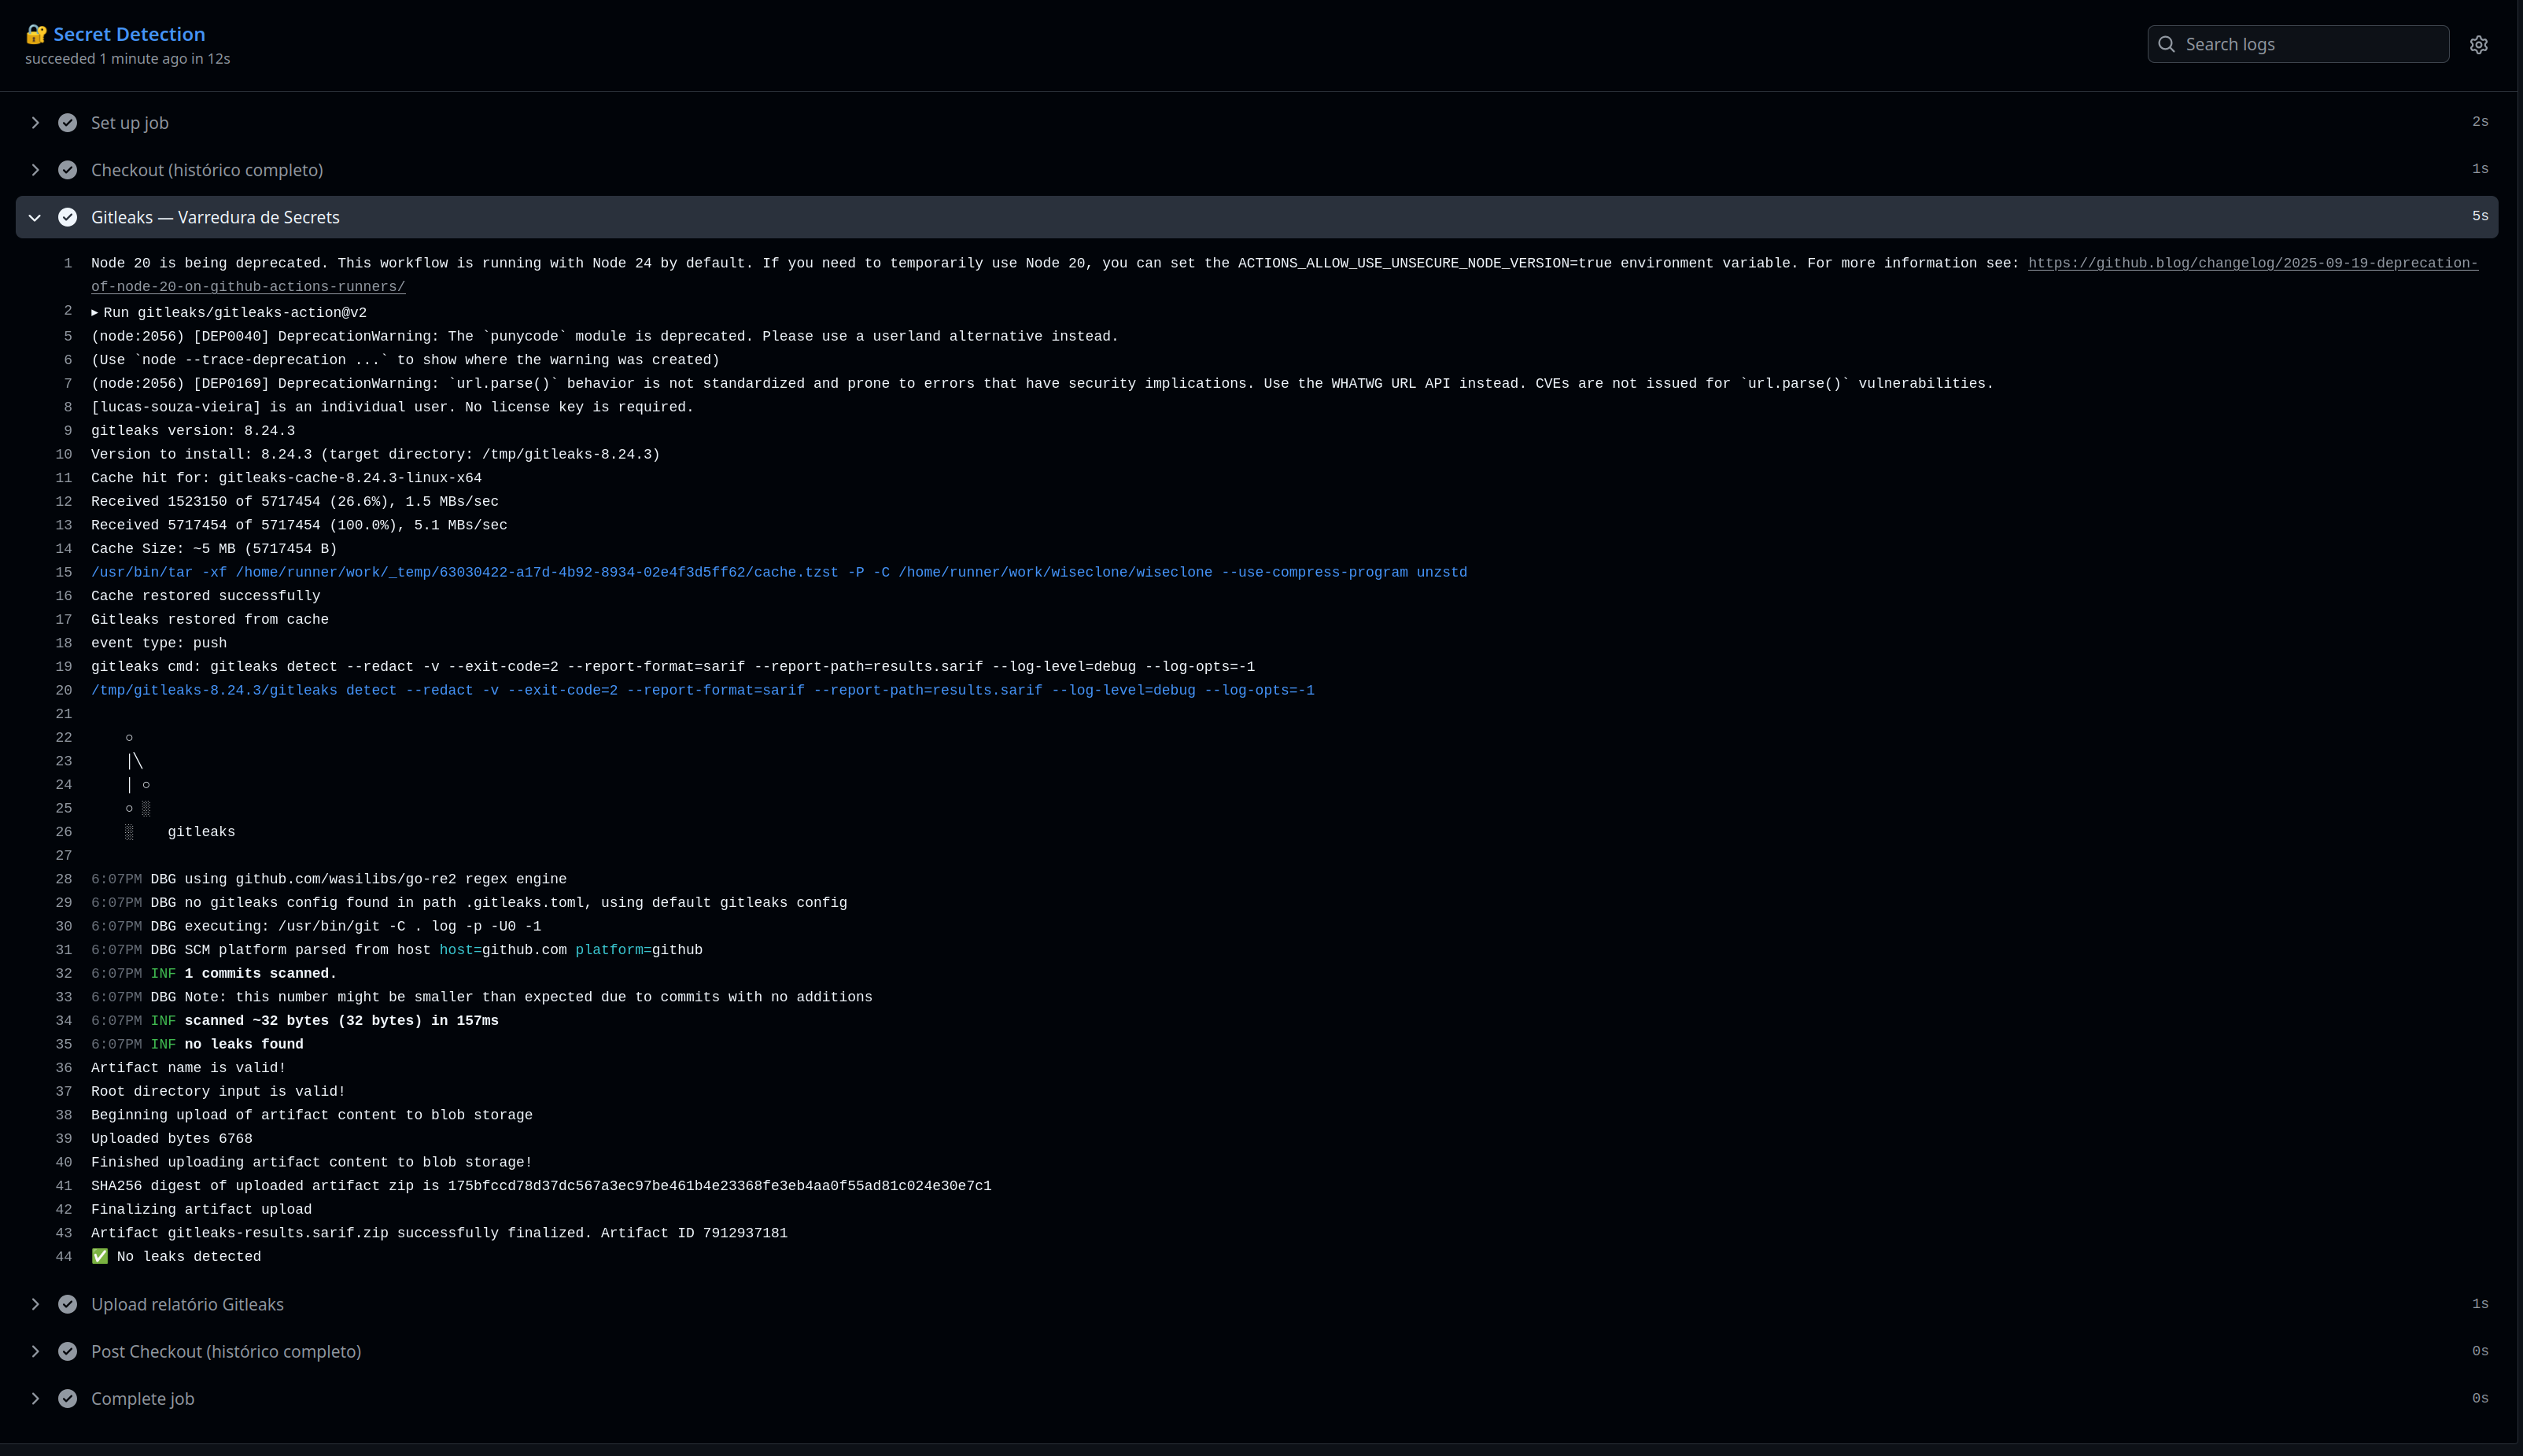
\includegraphics[width=0.8\textwidth]{images/gitleaks.png}
\caption{Saída do Gitleaks no Actions}
\label{fig:gitleaks}
\end{figure}

\begin{figure}[htbp]
\centering
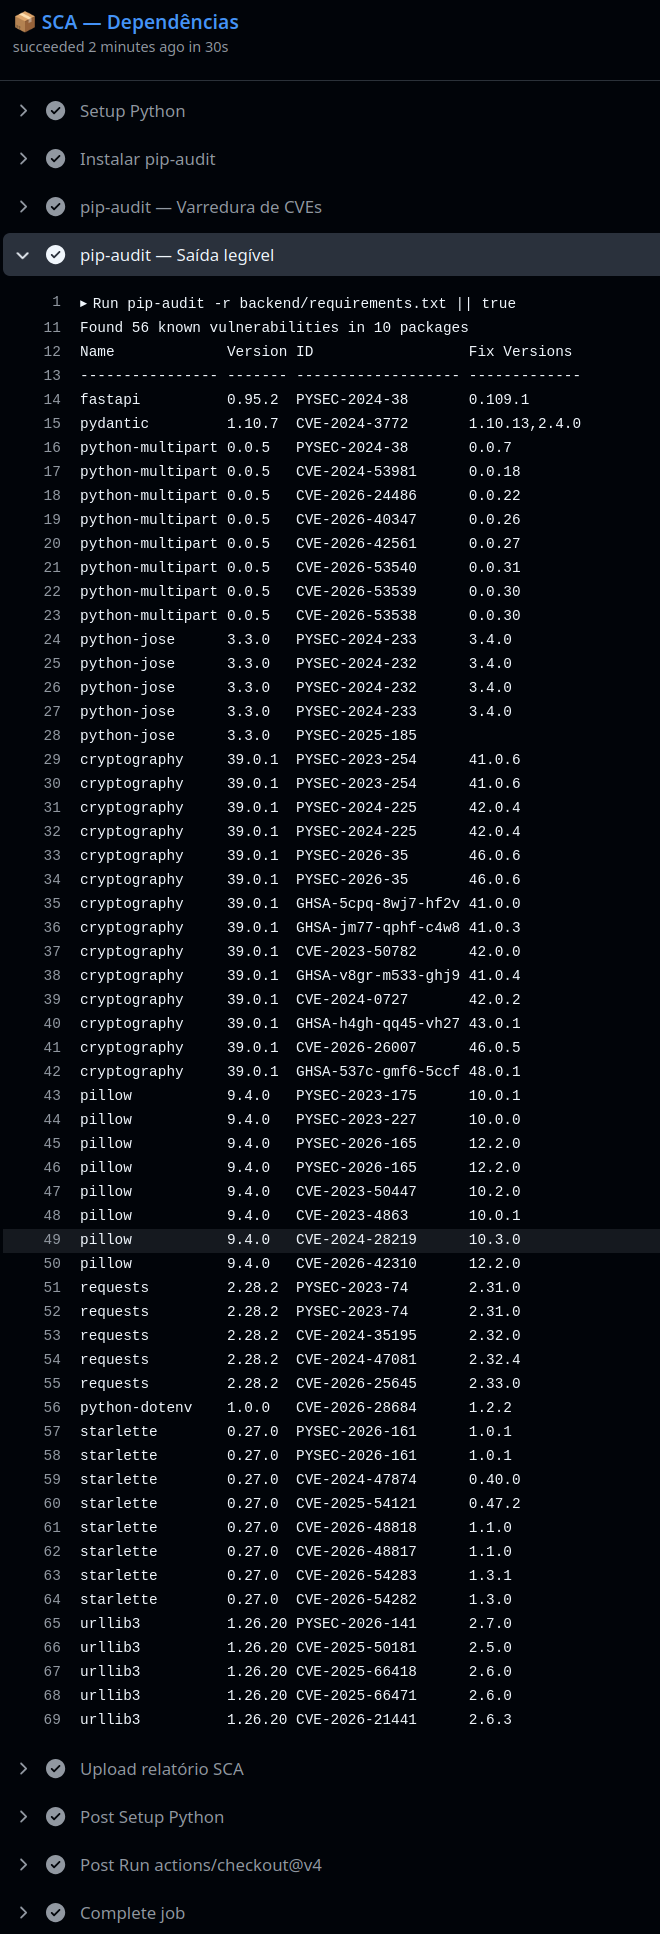
\includegraphics[height=11cm, keepaspectratio]{images/pip-audit.png}
\caption{Saída do pip-audit com as 56 vulnerabilidades}
\label{fig:pipaudit}
\end{figure}

\begin{figure}[htbp]
\centering
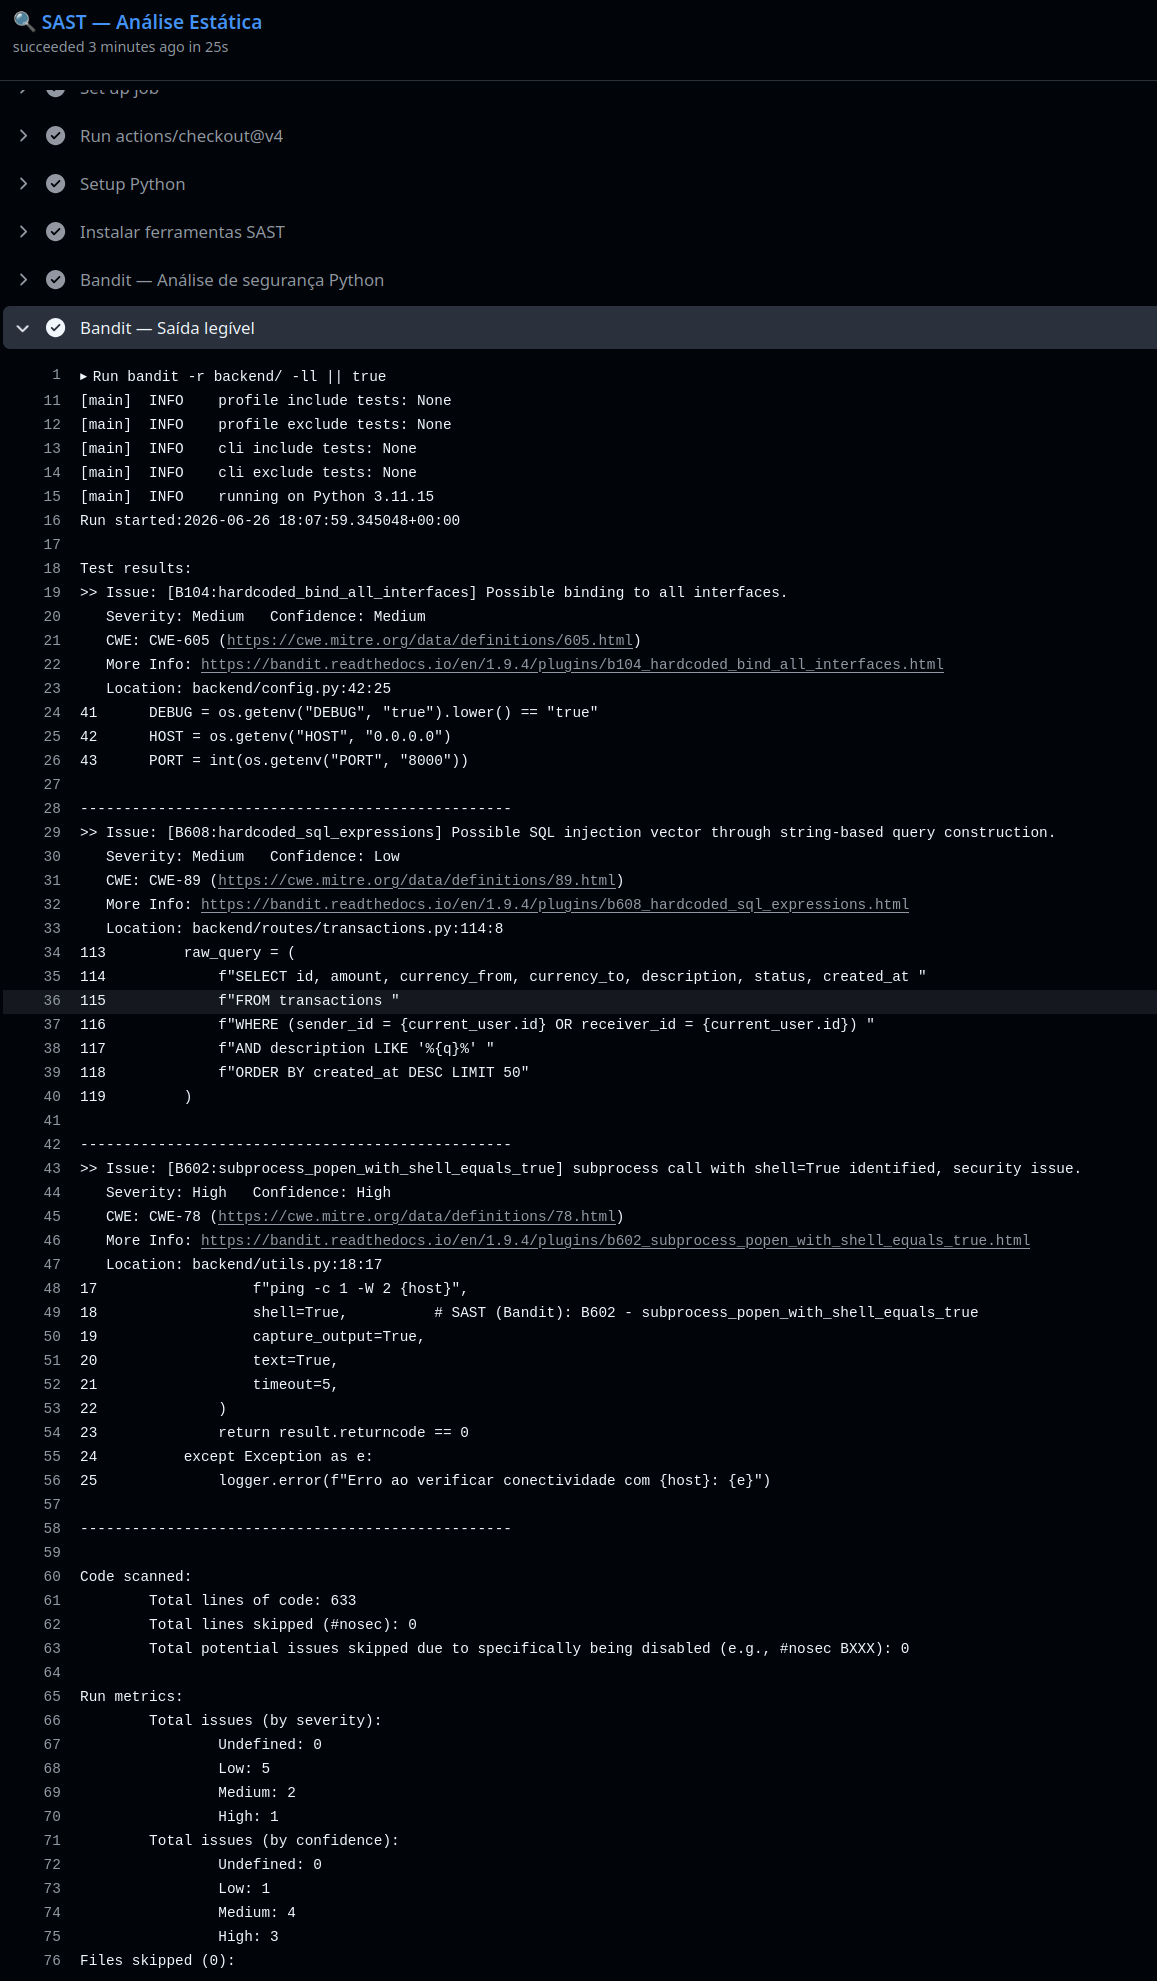
\includegraphics[width=0.8\textwidth]{images/bandit.png}
\caption{Saída do Bandit}
\label{fig:bandit}
\end{figure}

\begin{figure}[htbp]
\centering
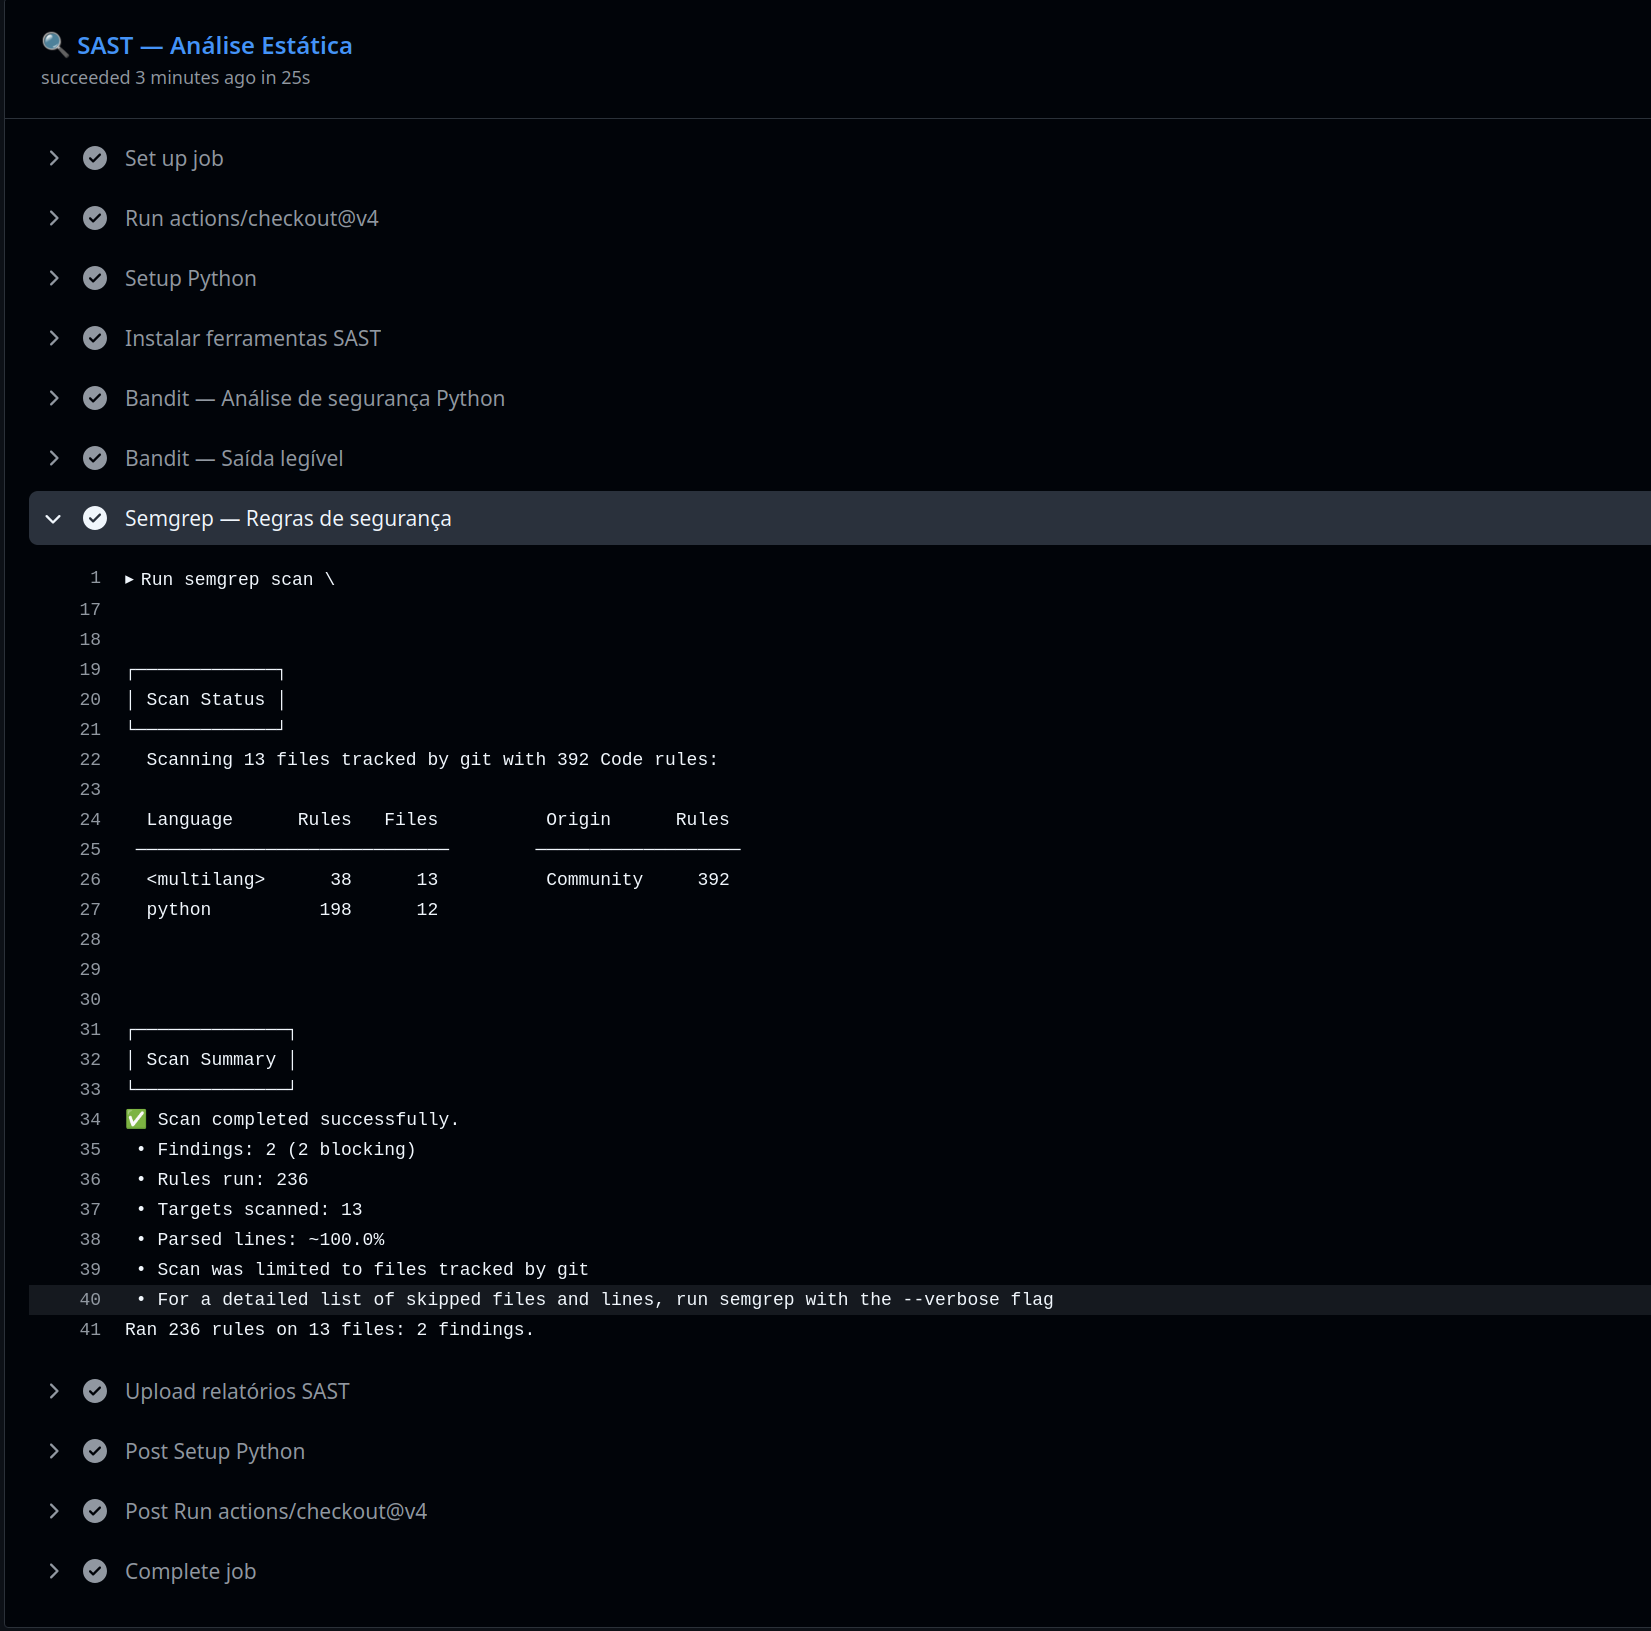
\includegraphics[width=0.8\textwidth]{images/semgrep.png}
\caption{Saída do Semgrep}
\label{fig:semgrep}
\end{figure}

\begin{figure}[htbp]
\centering
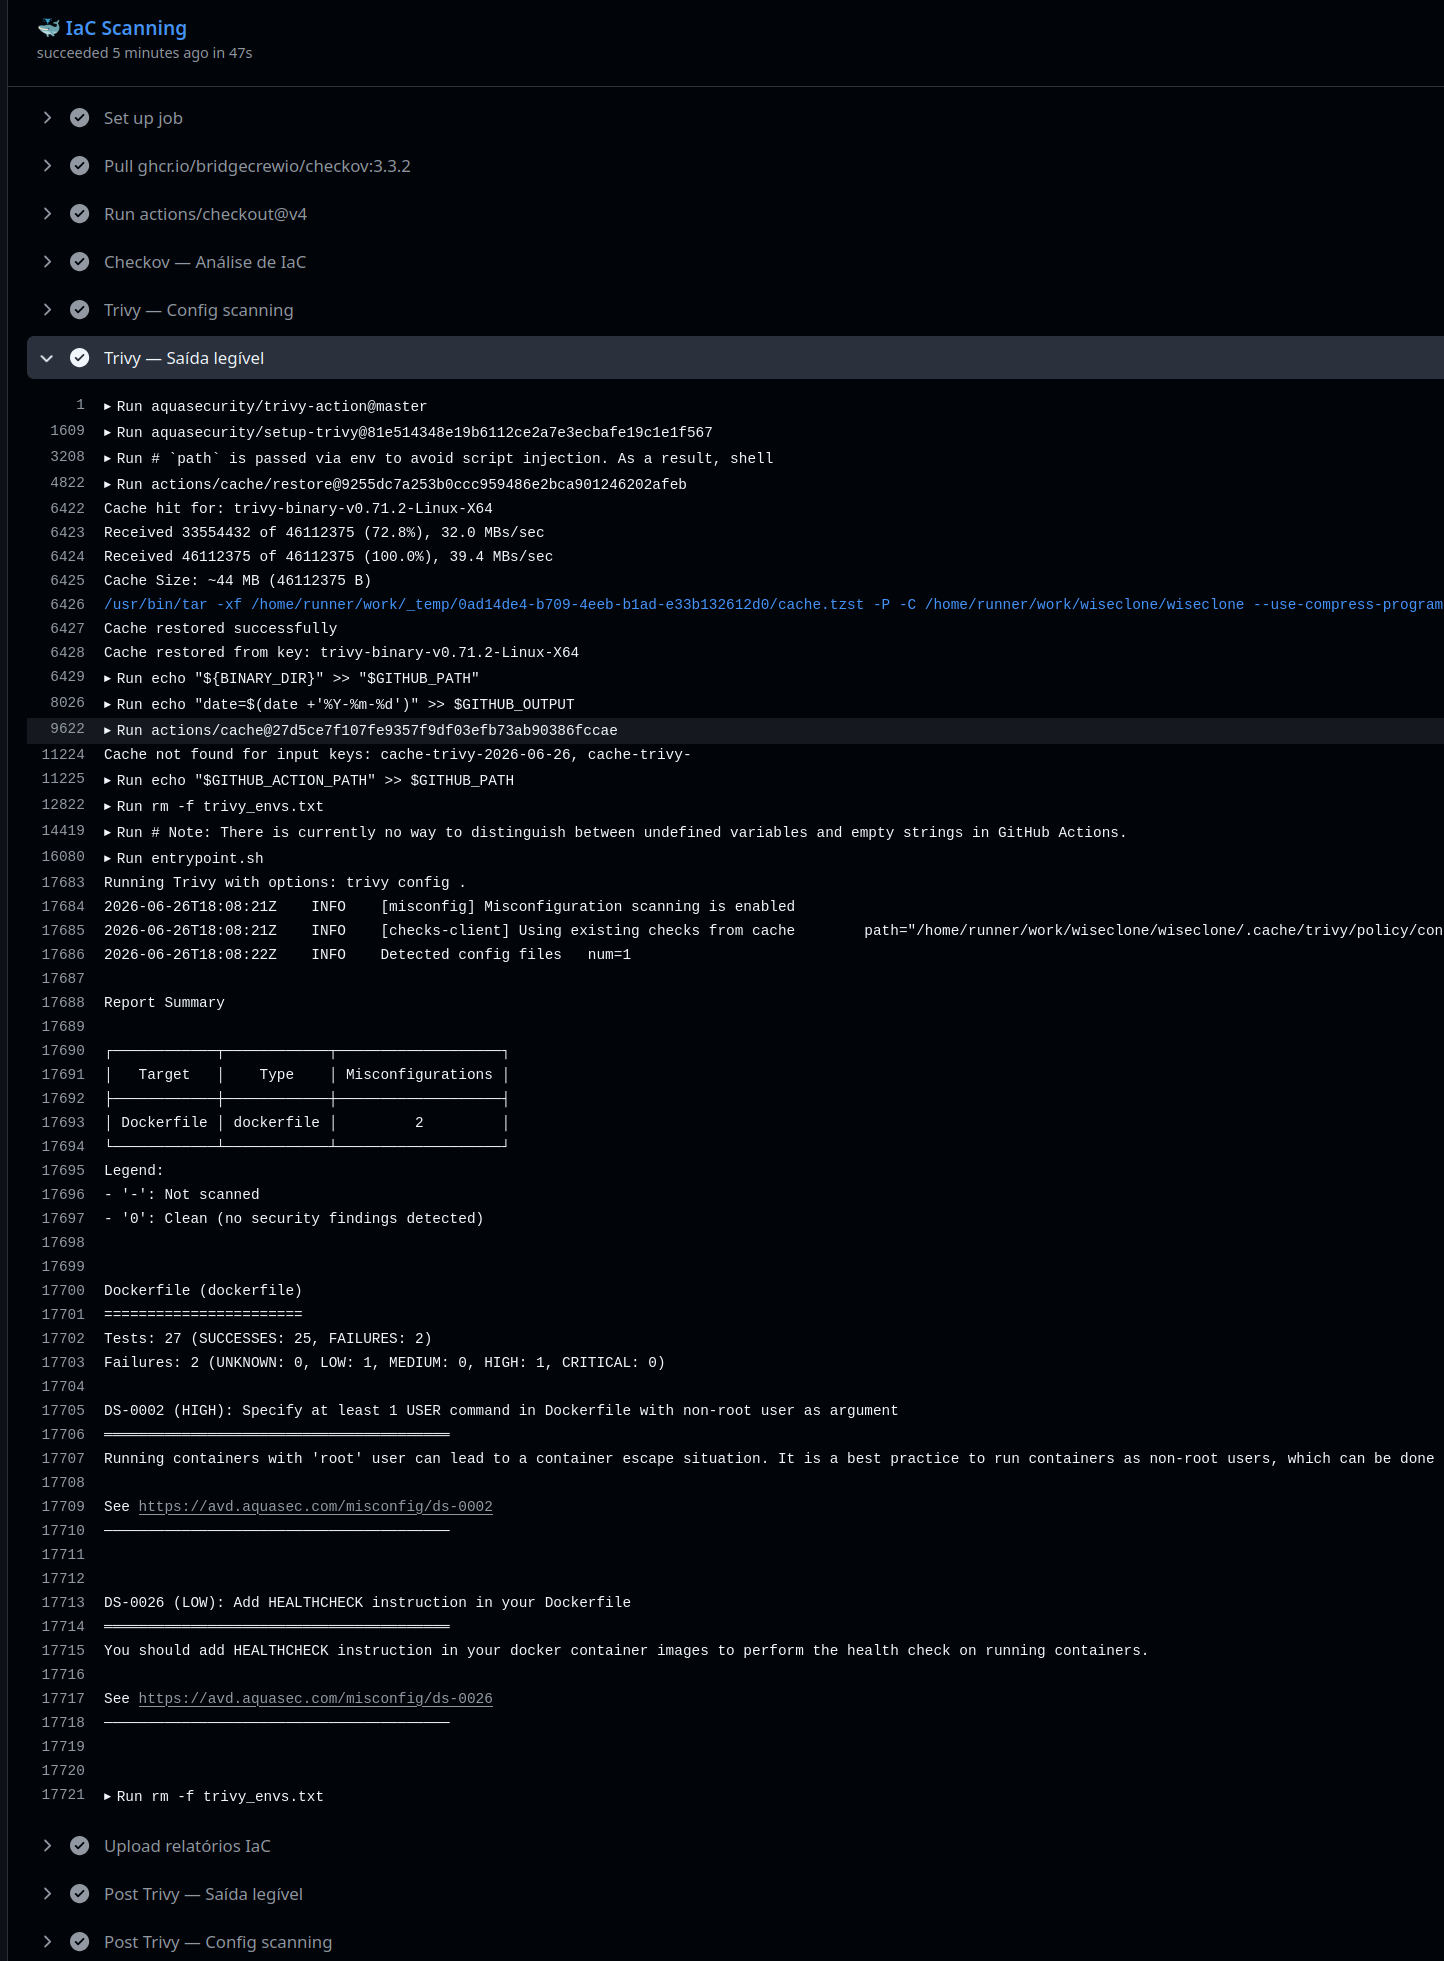
\includegraphics[width=0.8\textwidth]{images/checkov.png}
\caption{Saída do Trivy com análise do Dockerfile}
\label{fig:trivy}
\end{figure}

\begin{figure}[htbp]
\centering
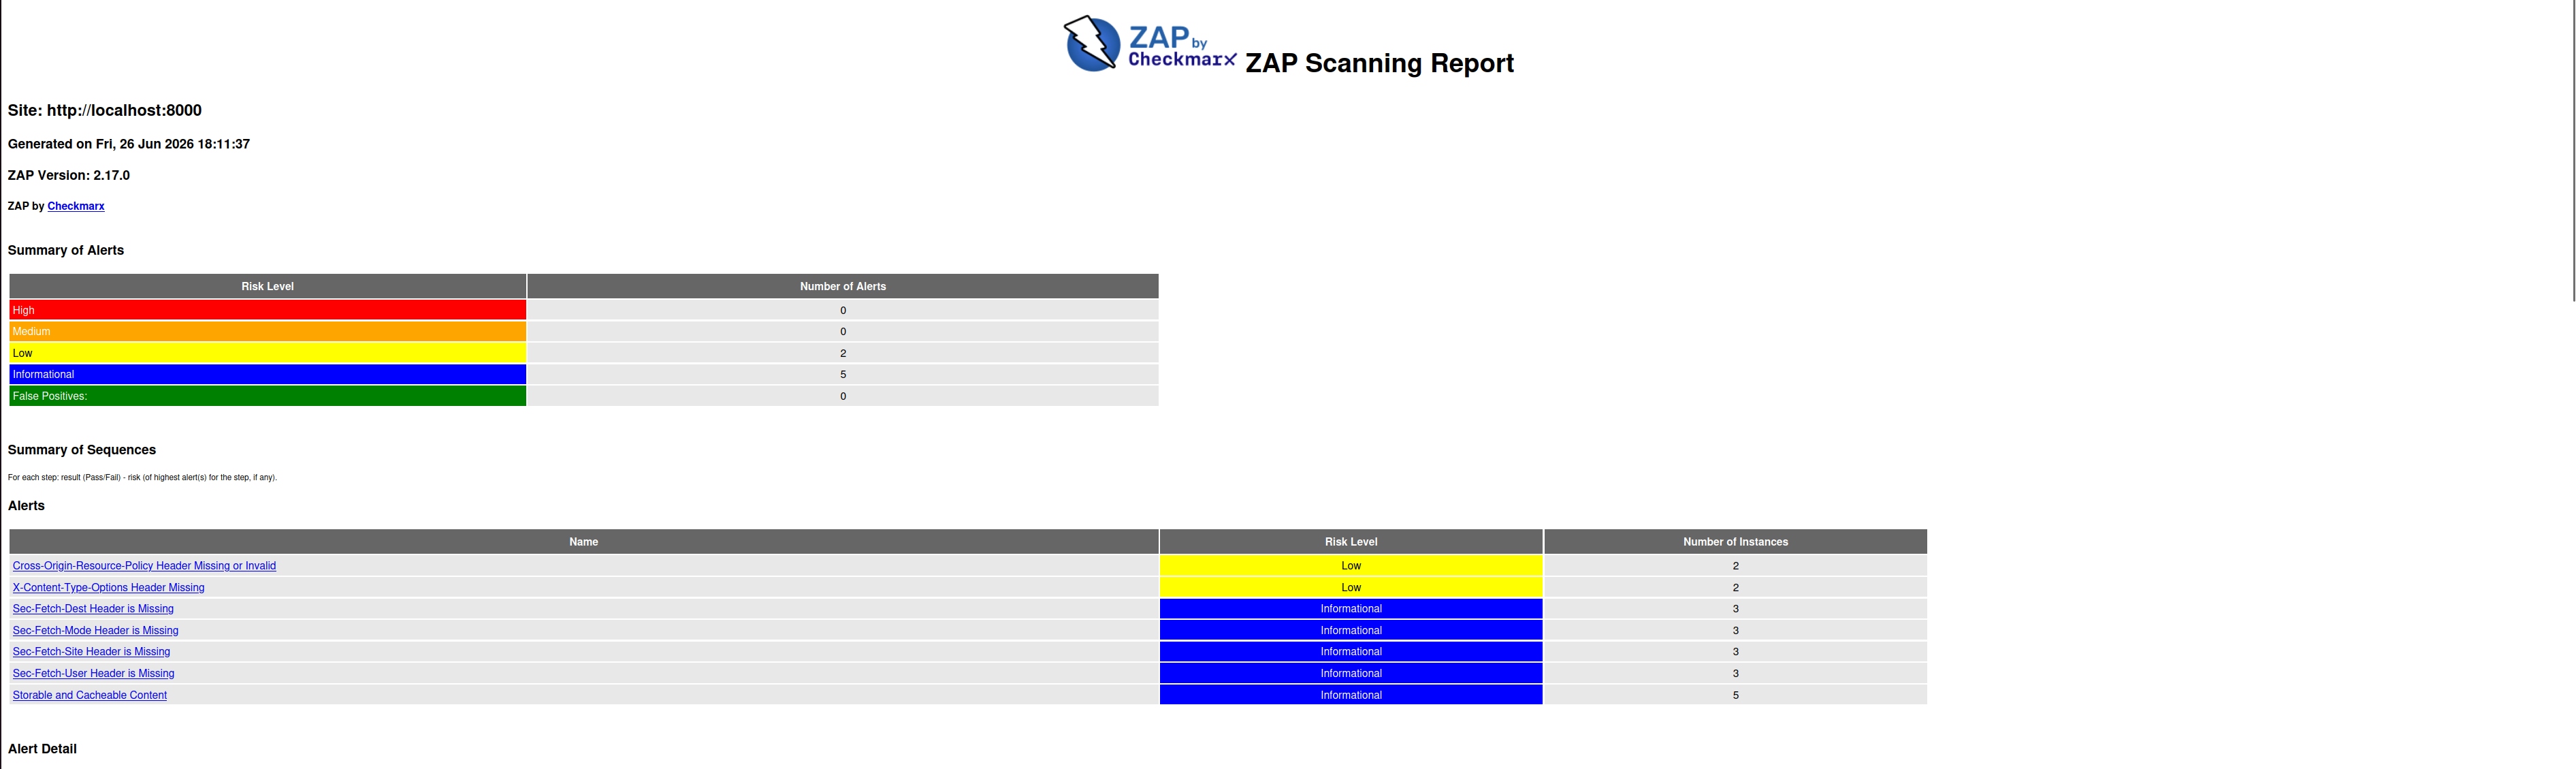
\includegraphics[width=0.8\textwidth]{images/zap.png}
\caption{Relatório OWASP ZAP}
\label{fig:zap}
\end{figure}

\end{document}
